\documentclass[varwidth=true, border=2pt]{standalone}
\usepackage{tikz}
\usepackage{nicefrac}

\begin{document}
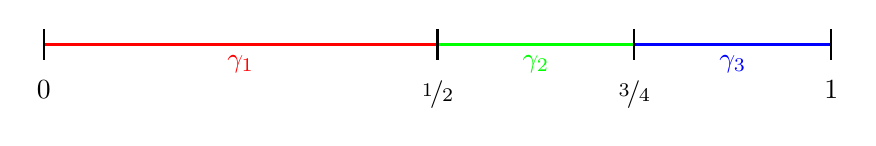
\begin{tikzpicture}
    \draw[very thick,red]   (0,0) -- (5,0) node [midway, below] {$\gamma_1$};
    \draw[very thick,green](5,0) -- (7.5,0) node [midway, below] {$\gamma_2$};
    \draw[very thick,blue] (7.5,0) -- (10,0) node [midway, below] {$\gamma_3$};

    \draw[thick] (0,0.2)   -- (  0,-0.2) node[label=below:$0$] {};
    \draw[thick] (5,0.2)   -- (  5,-0.2) node[label=below:$\nicefrac{1}{2}$] {};
    \draw[thick] (7.5,0.2) -- (7.5,-0.2) node[label=below:$\nicefrac{3}{4}$] {};
    \draw[thick] (10,0.2)  -- ( 10,-0.2) node[label=below:$1$] {};
\end{tikzpicture}
\end{document}
